\documentclass[12pt,a4paper]{ctexart}
\usepackage{amssymb}
\usepackage{amsmath}
\usepackage{graphicx}
\usepackage{float}
\usepackage{pythonhighlight}
\usepackage[linesnumbered,ruled]{algorithm2e}

\numberwithin{equation}{section}%公式按章节编号
\numberwithin{figure}{section}%图表按章节编号

\title{\heiti 基于tensor实现的神经网络}
\author{2333105 Ning Zhiheng}
\date{}
\begin{document}
\maketitle

\section{理论基础}
\subsection{矩阵求导}
\label{section:juzhenqiudao}
众所周知,对于实值标量函数$y=f(\boldsymbol{X})$
其中$y \in \mathbb{R}$,$\boldsymbol{X} \in \mathbb{R}^{p \times q}$,$ f: \mathbb{R}^{p \times q} \rightarrow \mathbb{R}$。
我们有下式成立:
\begin{equation}
    d y=\mathrm{tr}(\frac{\partial{f}}{\partial{\boldsymbol{X}}^T} d \boldsymbol{X}) \label {daoshu}
\end{equation}
由于没有既成的矩阵复合求导公式,并不能简单遵循实数求导的链式法则
认为$\frac{\partial{y}}{\partial{\boldsymbol{X}}}=\frac{\partial{f}}{\partial{\boldsymbol{G(X)}}} \frac{\partial{\boldsymbol{G(X)}}}{\partial{\boldsymbol{X}}}$,
其中$f: \mathbb{R}^{m \times n} \rightarrow \mathbb{R},\boldsymbol{G}:\mathbb{R}^{p \times q} \rightarrow \mathbb{R}^{m \times n}$是成立的。

下面我们从微分的本质来推导矩阵复合函数的求导法则,给定$y=f(\boldsymbol{M})$,
$\boldsymbol{M}=\boldsymbol{AXB}$,求$\frac{\partial{y}}{\partial{\boldsymbol{X}}}$
\begin{equation}
d y=\mathrm{tr}(\frac{\partial{f}}{\partial{\boldsymbol{M}}^T} d \boldsymbol{M})
                =\mathrm{tr}(\frac{\partial{f}}{\partial{\boldsymbol{M}}^T} \boldsymbol{A} d \boldsymbol{X} \boldsymbol{B} )
                =\mathrm{tr}( ( \boldsymbol{A}^T \frac{\partial{f}}{\partial{\boldsymbol{M}}} \boldsymbol{B}^T )^T d \boldsymbol{X})
\end{equation}
即$\frac{\partial{y}}{\partial{\boldsymbol{X}}}=  \boldsymbol{A}^T \frac{\partial{f}}{\partial{\boldsymbol{M}}} \boldsymbol{B}^T $。\\
(为了节省篇幅,本文后面给定的抽象函数都认为是实值标量函数),

\subsection{监督学习}
先回忆一下监督学习的范式,定义样本空间$\boldsymbol{X} \in \mathcal{X}$,标记空间$ \boldsymbol{Y} \in \mathcal{Y}$
以及包含了从$\mathcal{X}$到$\mathcal{Y}$的假设空间 $\mathcal{H}=\mathcal{X} \times \mathcal{Y}$,
同时考虑损失函数$\mathcal{Y} \times \mathcal{Y} \rightarrow \mathbb{R}$,$\boldsymbol{P}$为样本空间中$\mathcal{H}$的测度,我们要做的就是最小化损失函数,即
\begin{equation}
\min \limits_{\boldsymbol{w,b}}E_p({L(\boldsymbol{\hat{Y}},h_{\boldsymbol{w,b}}(\boldsymbol{X}))})
\end{equation}
其中,$\boldsymbol{\hat{Y}}$为真实值,$h \in \mathcal{H}$。\\
给定样本集$\mathcal{D}=\{(\boldsymbol{x_1},y_1),\ldots,(\boldsymbol{x_n},y_n)\}$,
其中$\boldsymbol{x_i} \in \mathbb{R}^d$, $y_i \in \mathbb{R}$, $ |\mathcal{D}|=n$。
并且$\mathcal{D}$中每个样本集都是独立从样本空间采样的,
我们有$\lim \limits_{n \rightarrow + \infty} \frac{1}{n} {L(\boldsymbol{\hat{Y}},h_{\boldsymbol{w,b}}(\boldsymbol{X}))}= E_p({L(\boldsymbol{\hat{Y}},h_{\boldsymbol{w,b}}(\boldsymbol{X}))})$,这是根据Hoeffding不等式给出的,
其中$\frac{1}{n} {L(\boldsymbol{\hat{Y}},h_{\boldsymbol{w,b}}(\boldsymbol{X}))}$是经验损失函数。\\
接着,问题便转换成优化经验损失函数,即:
\begin{equation}
    \boldsymbol{w,b}=\arg\min \limits_{\boldsymbol{w,b}}{L(\boldsymbol{\hat{Y}},h_{\boldsymbol{w,b}}(\boldsymbol{X}))}
\end{equation}
下面使用梯度下降法来求解这个问题(完整思想不再赘述,请读者自行查阅)。梯度下降法的核心是 \textbf{沿着梯度反方向的方向,函数局部下降最快}。
即可以通过迭代的方式,不断优化参数逼近最小值,表达式如下:
\begin{gather}
    \boldsymbol{w}^{(k+1)}=\boldsymbol{w}^{(k)}- \alpha \nabla_{\boldsymbol{w}} L \notag \\
    \boldsymbol{b}^{(k+1)}=\boldsymbol{b}^{(k)}- \alpha \nabla_{\boldsymbol{b}} L \label{tiduxiajiang}
\end{gather}
其中$\alpha$是步长,$\boldsymbol{w}^{(k)}$、$\boldsymbol{b}^{(k)}$是第$k$次迭代的参数。\\
按照上述流程,假如我们一直迭代,便可以得到函数取\textbf{全局最小值}时的参数$\boldsymbol{w,b}$。
细心的读者可能会发现,既然用这么简单的方法就可以求解,那为什么深度学习(神经网络)中还有如此多调参的“艺术”? \\
这需要解释三个核心的点:
\begin{itemize}
    \item [1)] 
    沿着梯度反方向函数值确实会减少,但如果$\alpha$太大,可能就可能适得其反,如图\ref{步长选择策略},
    所以正确的调参模式应该为:
    \begin{align}
        \boldsymbol{w}^{(k+1)}&=\arg \min \limits_{\boldsymbol{w}}L(\boldsymbol{w}^{(k)}- \alpha \nabla_{\boldsymbol{w}} L) \notag  \\
        \boldsymbol{b}^{(k+1)}&=\arg \min \limits_{\boldsymbol{b}} L(\boldsymbol{b}^{(k)}- \alpha \nabla_{\boldsymbol{b}} L) \label{tiduxiajiang1}
    \end{align}
    由于$\boldsymbol{w,b}$是变值,每一次迭代取得最小值的$\alpha$便不是唯一的,可以使用精确步长搜索方法确定$\alpha$。
    为了简单实践,本文采用简单批量随机梯度下降法,并设置$\alpha=0.01$,这可以近似保证函数的值呈现下降趋势。
    \item [2)] 
    简单梯度下降法是一个贪心的算法,因此不能保证函数在\textbf{全局}上下降得最快,若求解一个可解问题所需的时间很多,
    那么算法便失去了意义,这时候我们说这个问题是“无解”的。
    \item[3)]
    通常来说我们希望损失函数为凸函数,因为梯度下降法一旦收敛便是该函数的全局最小值点;
    而对于非凸函数来说,由于存在多个局部最小值点,一旦算法跳进局部陷阱,便很难跳出来。
\end{itemize}
所以为了更好更快地使函数收敛到最小值,神经网络超参数调优也是一个值得研究的领域。
\begin{figure}[!h] %h表示就在此处插入。
    \centering % 居中
    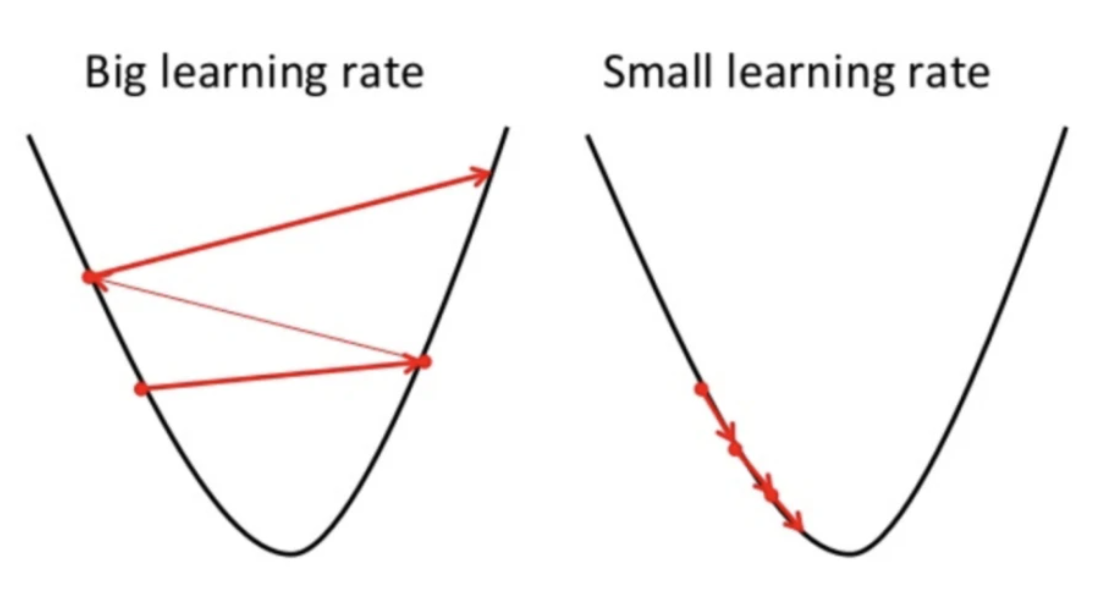
\includegraphics[scale=0.6]{tiduxiajiang.png} %在tex所在文件夹下面创建一个名为figs的文件夹,并把所有要用的照片放这里。当然你也可以选择使用绝对路径。
    \caption{步长选择策略}
    \label{步长选择策略} % 为每个图片设置一个标识
    \end{figure}
\section{网络结构}
\subsection{全连接层}
首先给出全连接层的数学模型,设输入该层的数据为$\boldsymbol{X} \in  \mathbb{R}^{n \times d}$,权重矩阵为$\boldsymbol{W} \in  \mathbb{R}^{ d \times p }$,
,偏置向量为$\boldsymbol{b} \in \mathbb{R}^{1 \times p} $,输出为$ \boldsymbol{Y} \in \mathbb{R}^{n \times p}$。则:
\begin{equation}
\boldsymbol{Y}_{n \times p}=\boldsymbol{X}_{n \times d}\boldsymbol{W}_{d \times p}+\boldsymbol{1}_{n \times 1}\boldsymbol{b}_{1 \times p}
\end{equation}
这实际完成了特征从$d$维空间到$p$维空间的映射。
\subsubsection{前向传播}
因此,我们可以写出前向传播对应的函数:
\begin{python}
def forward(self, x):
    self.x = x
    sample_dim = x.shape[0]
    self.tensor_one = torch.ones([sample_dim, 1], dtype=torch.float64)
    x = torch.mm(x, self.w) + torch.mm(self.tensor_one, self.b)
    return x
\end{python}
\subsubsection{反向传播}
根据\ref{section:juzhenqiudao},容易给出$L$对$\boldsymbol(W,b,X)$的偏导:
\begin{gather}
    \nabla_{\boldsymbol{W}} L= \boldsymbol{X}^T \frac{\partial{L}}{\partial{\boldsymbol{Y}}} \notag \\
    \nabla_{\boldsymbol{b}} L =\boldsymbol{1_{n \times 1}}^T \frac{\partial{L}}{\partial{\boldsymbol{Y}}} \notag \\
    \nabla_{\boldsymbol{X}} L =\frac{\partial{L}}{\partial{\boldsymbol{Y}}} \boldsymbol{W}^T 
\end{gather}
因此我们可以写出反向传播对应的函数:
\begin{python}
def backward(self, top_gard):
    self.dw = torch.mm(self.x.transpose(0, 1), top_gard)
    self.db = torch.mm(self.tensor_one.transpose(0, 1), top_gard)
    bottom_gard = torch.mm(top_gard, self.w.transpose(0, 1))
    return bottom_gard
\end{python}
\subsection{Relu层}
给出$\mathrm{Relu}$表达式:
\begin{equation}
\mathrm{Relu}(\boldsymbol{X})=\max(\boldsymbol{X},0)
=\left \{ 
\begin{aligned}
\boldsymbol{X} \quad &\boldsymbol{X} \geq 0 \\
0 \quad &otherwise
\end{aligned}
    \right
    .
\label{relu}
\end{equation}
给出Relu的图像,如下图所示:
\begin{figure}[!h] %h表示就在此处插入。
    \centering % 居中
    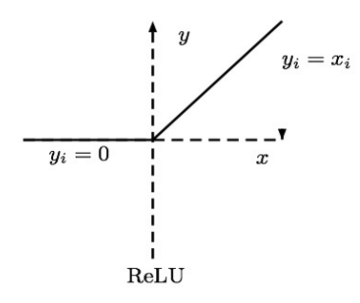
\includegraphics[scale=0.7]{relu.png} %在tex所在文件夹下面创建一个名为figs的文件夹,并把所有要用的照片放这里。当然你也可以选择使用绝对路径。
    \caption{$\mathrm{Relu}$函数示意图}
    \label{fig} % 为每个图片设置一个标识
    \end{figure}

\noindent 可以看到这是一个非线性的函数,可以作为全连接层的激活函数。
\subsubsection{前向传播}
因此,我们可以写出前向传播对应的函数:
\begin{python}
def forward(self, x):
    self.x = x
    x = torch.maximum(x, torch.tensor([0.0]))
    return x
\end{python}
\subsubsection{反向传播}
根据式\eqref{relu},求出$\mathrm{Relu}(x)$的导数:
\begin{equation}
\mathrm{Relu}'(x)=\left \{ 
    \begin{aligned}
    1 \quad &x \ge 0 \\
    0 \quad &otherwise
    \end{aligned}
    \right .
\end{equation}
接着写出反向传播对应的公式:
\begin{equation}
\nabla_{\boldsymbol{X}} L= \nabla_{\boldsymbol{Y}} L \circ \mathrm{Relu}'(\boldsymbol{X})
=\left \{ 
    \begin{aligned}
    \nabla_{\boldsymbol{Y}} L \quad &\boldsymbol{X} \ge 0 \\
    0 \quad &otherwise
    \end{aligned}
    \right .
\end{equation}
其中$\circ$为哈达玛积。\\
因此我们可以写出反向传播对应的函数:
\begin{python}
def backward(self, top_grad):
    bottom_grad = top_grad
    bottom_grad[self.x < 0] = 0
    return bottom_grad
\end{python}
\subsection{softmax层}
给出多分类情况下大家常用的$\mathrm{softmax}$表达式:
\begin{equation}
\mathrm{softmax}(\boldsymbol{x})=\frac{\exp (\boldsymbol{x})}{\sum_{i=1}^d \exp(\boldsymbol{x})}
=\frac{\exp (\boldsymbol{x})}{\boldsymbol{1}^T \exp(\boldsymbol{x})}
\end{equation}
其中$x \in \mathbb{R}^d$,可以看到本质上就是一个将向量中每个元素映射到区间$[0,1]$的函数,即$f:\mathbb{R}^n \rightarrow \mathbb{R}_{[0,1]}$。
若$\boldsymbol{X} \in \mathbb{R}^{n \times d}$为矩阵,则公式变为:
\begin{align}
    \mathrm{softmax}(\boldsymbol{X})&=(\mathrm{softmax}(\boldsymbol{x_1}),\dots,\mathrm{softmax}(\boldsymbol{x_n}))^T \notag \\
    &=\mathrm{diag}^{-1}\{\exp(\boldsymbol{X})\boldsymbol{1}\} \exp(\boldsymbol{X}) \label{softmax}
\end{align}
其中$\boldsymbol{X}=(\boldsymbol{x_1},\dots,\boldsymbol{x_n})^T$。\\
读者看到这里可能会感觉疑惑,$\mathrm{softmax}(\boldsymbol{X})$与$\boldsymbol{X}$都是矩阵的形式,
而我们从未提及$\frac{\partial{\mathrm{softmax}(\boldsymbol{X})}}{\partial{\boldsymbol{X}}}$这样矩阵对矩阵的求导形式,
该怎么办?\\
事实上,在神经网络中,$\mathrm{softmax}$与交叉熵函数是成双成对出现的。
为了便于后续说明,在此先给出交叉熵函数的数学表达式:
\begin{equation}
L(\boldsymbol{\hat{y}},\boldsymbol{y})= \sum_{i=1}^d -\hat{y_i} \log(y_i)=-\boldsymbol{\hat{Y}}^T \log(\boldsymbol{Y}) \label{jiaochashang}
\end{equation}
其中$\boldsymbol{y}=(y_1,\dots,y_d)^T$,$\boldsymbol{\hat{y}}=(\hat{y_1},\dots,\hat{y_d})^T$,
$\hat{\boldsymbol{Y}}= (\boldsymbol{\hat{y_1}},\dots,\boldsymbol{\hat{y_n}})^T$,
$\hat{y_i}
=\left \{ 
    \begin{aligned}
    1 \quad &i=k \\
    0 \quad &i \neq k
    \end{aligned}
    \right .
$,表明样本属于第$k$类。\\
考察式\eqref{jiaochashang},容易发现其为一个标量。
于是尝试把式\eqref{softmax}与式\eqref{jiaochashang}结合起来以实现标量$L$对矩阵$\boldsymbol{X}$的求导。
至此,给出重新定义的$\mathrm{softmax}$层的公式:
\begin{align}
L(\boldsymbol{\hat{Y}},h(\boldsymbol{X}))
&= \sum_{i=1}^n -\boldsymbol{\hat{y_i}} \log(\mathrm{softmax}(\boldsymbol{x_i}))
=\mathrm{tr}(-\boldsymbol{\hat{Y}} \log\mathrm{softmax}(\boldsymbol{X})) \notag \\
&=-\mathrm{tr}(\boldsymbol{\hat{Y}} \log(\mathrm{diag}^{-1}\{\exp(\boldsymbol{X})\boldsymbol{1}\}))
\end{align}
\subsubsection{前向传播公式}
因此,我们可以写出前向传播对应的函数(这包含了损失函数):
\begin{python}
def softmax(x):
    x = torch.exp(x)
    x = x / torch.sum(x, dim=1, keepdim=True)
    return x

def forward(self, x):
    self.x = x
    self.outputs = softmax(x)
    return self.outputs
    def get_loss(self, true_targets):
        assert true_targets.shape[0] == self.x.shape[0]
        self.true_targets_encode = self.encode_targets(true_targets)
        total_loss = 0.0
        for i, true_target in enumerate(true_targets):
            loss = self.sample_loss(i)
            total_loss += loss
        total_loss = total_loss / true_targets.shape[0]
        return total_loss

def sample_loss(self, index):
    return -torch.dot(torch.log(self.outputs[index]), self.true_targets_encode[index])
\end{python}
\subsubsection{反向传播公式}
同样的,给出反向传播对应的公式:
\begin{align}
\nabla_{\boldsymbol{X}} L 
= \frac{1}{m} (\mathrm{softmax}(\boldsymbol{X})-\boldsymbol{\hat{Y}})
= \frac{1}{m} (\boldsymbol{Y-\hat{Y}})
\end{align}
因此我们可以写出反向传播对应的函数:
\begin{python}
def backward(self):
    sample_count = self.outputs.shape[0]
    bottom_grad = (self.outputs - self.true_targets_encode) / sample_count
    return bottom_grad
\end{python}
\end{document}
